\section{Results}

\begin{frame}{6.1 - Forecast exercise}
	\begin{itemize}
		\item sequential sample: start from 1993m7 - 2016m7, then increase sequentially by one month, for 36 months (3 years)
		\item for each sample: produce forecasts at $t+1$, $t+2$, $t+3$ and $t+4$
		\item forecasts are produced for GDP and all features in $x_t$
		\item for each model, sample, horizon and features, compute RMSE = $\sqrt{(x_{t+h} - \hat{x}_{t+h})^2}$
		\item consider the average RMSE over the different samples
	\end{itemize}	
\end{frame}

\begin{frame}{6.2 - Dynamic factors: illustration}
	\begin{figure}[h]
		\centering
		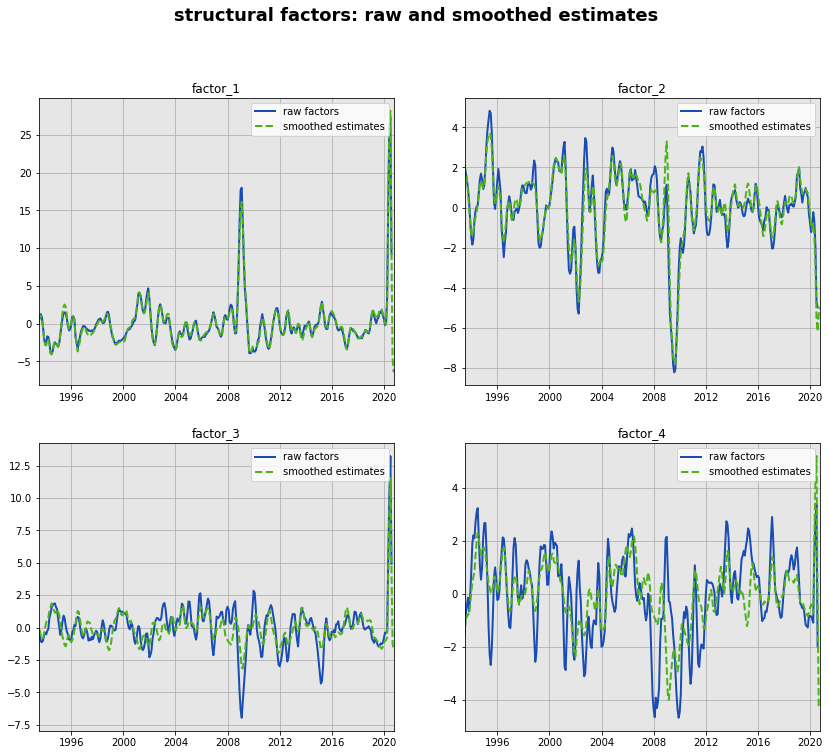
\includegraphics[width=.7\linewidth]{im1}
	\end{figure}
\end{frame}

\begin{frame}{6.3 - GDP predictions: all models, all horizons}
\begin{figure}[h]
	\centering
	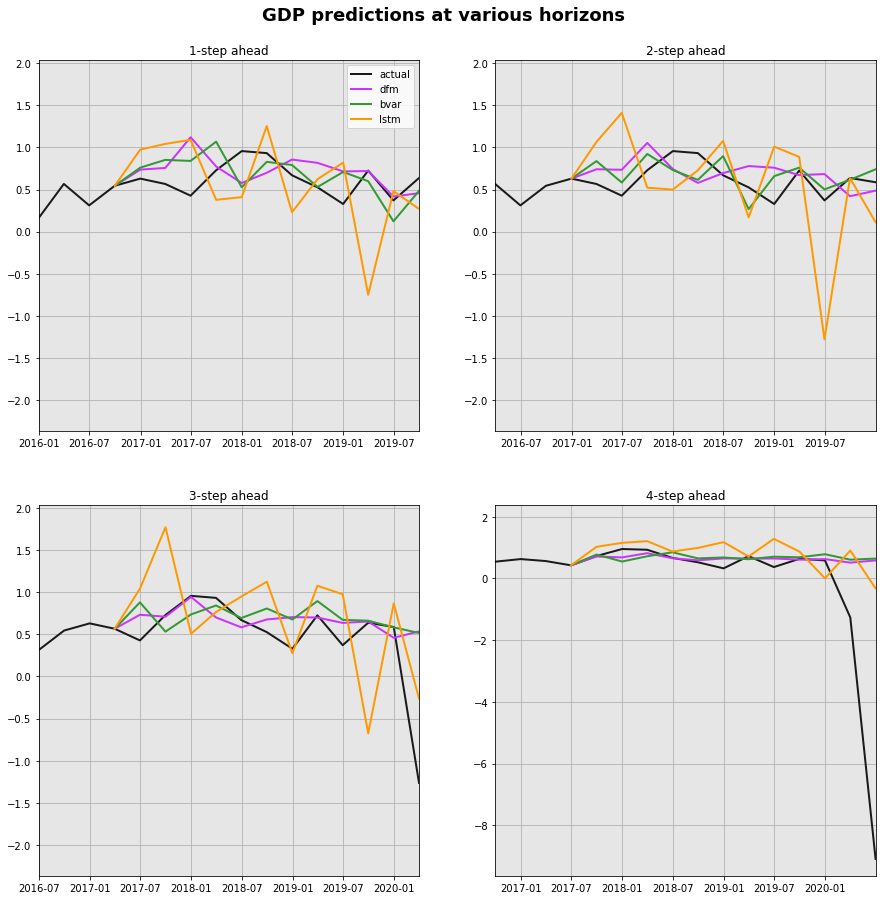
\includegraphics[width=.6\linewidth]{im2}
\end{figure}
\end{frame}

\begin{frame}{6.4 - GDP predictions: RMSE tables}
\begin{figure}[h]
	\centering
	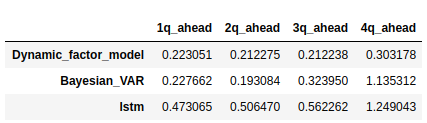
\includegraphics[width=0.8\linewidth]{im3}
\end{figure}
\end{frame}

\begin{frame}{6.5 - Feature predictions: all models, one quarter ahead}
\begin{figure}[h]
	\centering
	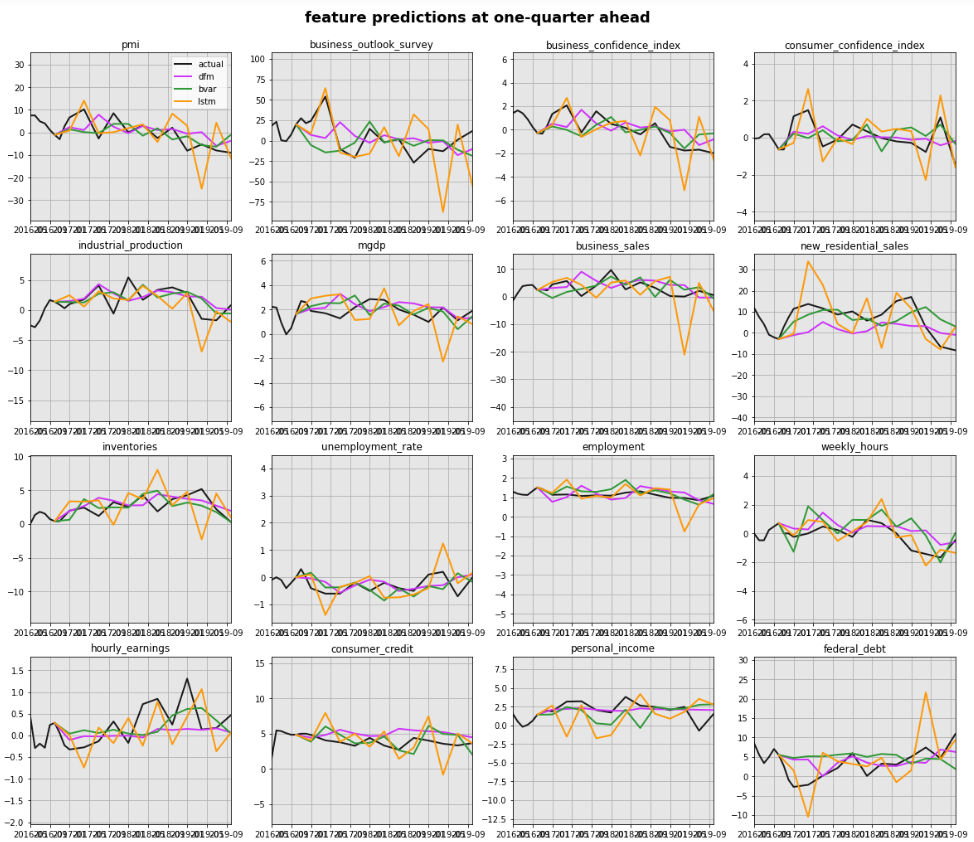
\includegraphics[width=0.8\linewidth]{im4}
\end{figure}
\end{frame}

\begin{frame}{6.6 - feature predictions: RMSE tables}
\begin{figure}[h]
	\centering
	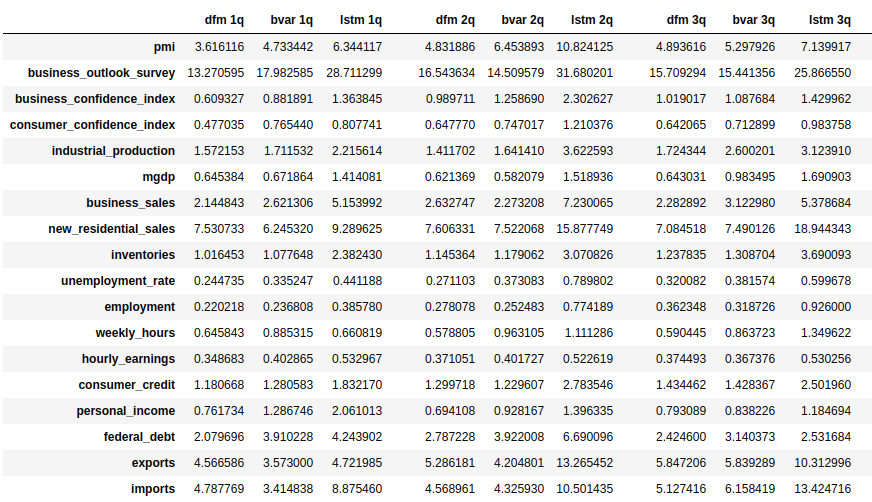
\includegraphics[width=1\linewidth]{im5}
\end{figure}
\end{frame}












